% !TeX root = ../build/main.tex

In the Vocdoni Z system, a vote comprises several components that work together to ensure secure, private, and verifiable voting. These components are:

\begin{enumerate}
	\item Process Identifier
	\item Census Proof
	\item Identity Commitment
	\item Nullifier
	\item Encrypted Ballot and Zero-Knowledge Proof (ZKP)
	\item Signature	
\end{enumerate}

Below, we detail each component and its role in the voting process.

\begin{enumerate}
	\item \textbf{Process Identifier} \\
	
			The \textbf{Process Identifier} (\texttt{ProcessId}) is a unique 32-byte number that uniquely identifies a specific voting process within the Vocdoni Z ecosystem. It encapsulates essential information, including the rules and constraints for ballots and the unique identifier of the Vocdoni Z blockchain instance.\\
			
	\item \textbf{Census Proof} \\
			
			The \textbf{Census Proof} serves as the voter's identity verification mechanism, ensuring that only eligible voters can participate. Depending on the process configuration, the voter provides:
			\begin{itemize}
				\item \textbf{Merkle Tree-Based Proof}: A Merkle proof showing inclusion in the census.
				\item \textbf{Credential Service Provider (CSP)}: A credential issued by a trusted third party. \\
			\end{itemize}
			
	\item \textbf{Identity Commitment}\\
	
			The \textbf{Commitment} $C$ is used to prevent a voter from registering multiple nullifiers and to avoid collisions if different voters choose the same secret.
			
			$$ C = \text{Hash} (\text{Address} || ProcessId || s). $$
			
			\begin{itemize}
				\item \textbf{Stored in State Merkle Tree (SMT)}: Indexed by the voter's address.
				\item \textbf{Prevents Multiple Registrations}: Each address can have only one commitment, ensuring a voter cannot register multiple secrets.
				\item \textbf{Collision Resistance}: Including the address in $C$ ensures that commitments are unique even if voters choose the same secret $s$.
			\end{itemize}
			
			The secret $s$ can be implemented from different ways or a combination of them, such as:
			
			\begin{itemize}
				\item A secure enough Password introduced by the user.
				\item A signature of a specific text.
				\item A random input that the user must store to allow potential vote overwrite.\\
			\end{itemize}
	
	\item \textbf{Nullifier} \\
	
			The \textbf{Nullifier} $N$ is a 32-byte hash used to:
			
			\begin{itemize}
				\item \textbf{Prevent Double Voting}: Ensures each voter can cast only one vote or overwrite their previous vote.
				\item \textbf{Allow Vote Overwriting}: Voters can submit a new vote with the same nullifier to replace their previous vote.
				\item \textbf{Provide Anonymity}: Cannot be linked back to the voter's identity without knowledge of the secret $s$.
			\end{itemize}
		
			$$ N = \text{Hash}(\text{C} || s) $$ 
			
	\item \textbf{Encrypted Ballot and Zero-Knowledge Proof (ZKP)} \\
	
			The ballot contains the voter's selections encoded according to the ballot protocol rules. To ensure privacy, the ballot is encrypted using the ElGamal cryptosystem over elliptic curves, which allows homomorphic combination of encrypted votes.
			
			\textbf{Encryption process}:
			
			\begin{itemize}
				\item The voter's choice $m$ is encoded as a point on the elliptic curve.
				\item The voter selects a random scalar $k \in [1, n-1]$, where is the order of the elliptic curve group.
				\item Compute the ciphertext components:
					\begin{itemize}
						\item $C_1 = k \cdot G$
						\item $C_2 = M + k \cdot H$
					\end{itemize}
				\item The ciphertext is the pair $(C_1, C_2)$.
			\end{itemize}


			\textbf{Zero-Knowledge Proof (ZKP)}:
			
			The voter generates a ZKP to prove the correctness of the ballot and encryption process:
			
			\begin{enumerate}
				\item \textbf{Correctness of Encryption}: Ensures the ciphertext $(C_1, C_2)$ is correctly computed from the plaintext message $M$ and random scalar $k$.
				\item \textbf{Compliance with Ballot Protocol Rules}: The plaintext vote adheres to the ballot protocol constraints, such as valid choices and allowed number of selections.
				\item \textbf{Correct Computation of Commitment and Nullifier}:
						\begin{itemize}
							\item \textbf{Commitment}: $C = \text{Hash} (\text{Address} || ProcessId || s).$
							\item \textbf{Nullifier}: $N = \text{Hash}(\text{C} || s)$.
							\item The voter knows the secret linking the commitment and nullifier.
						\end{itemize}
			\end{enumerate}
		
			\textbf{Inputs to the ZKP Circuit}:
			
			\begin{itemize}
				\item \textbf{Public Inputs}:
						\begin{itemize}
							\item Encrypted Ballot $(C_1, C_2)$.
							\item Ballot Protocol Configuration.
							\item Encryption Parameters.
							\item Voter's Weight
							\item Commitment $C$.
							\item Nullifier $N$.
						\end{itemize}
				\item \textbf{Private Inputs}:
						\begin{itemize}
							\item Plaintext Vote $m$.
							\item Secret $s$.
							\item Random Scalar $k$.
							\item Voter's Address (used internally in the computation of $C$).
						\end{itemize}
			\end{itemize}
		
	\begin{figure}[H]
		\centering
		\fbox{
			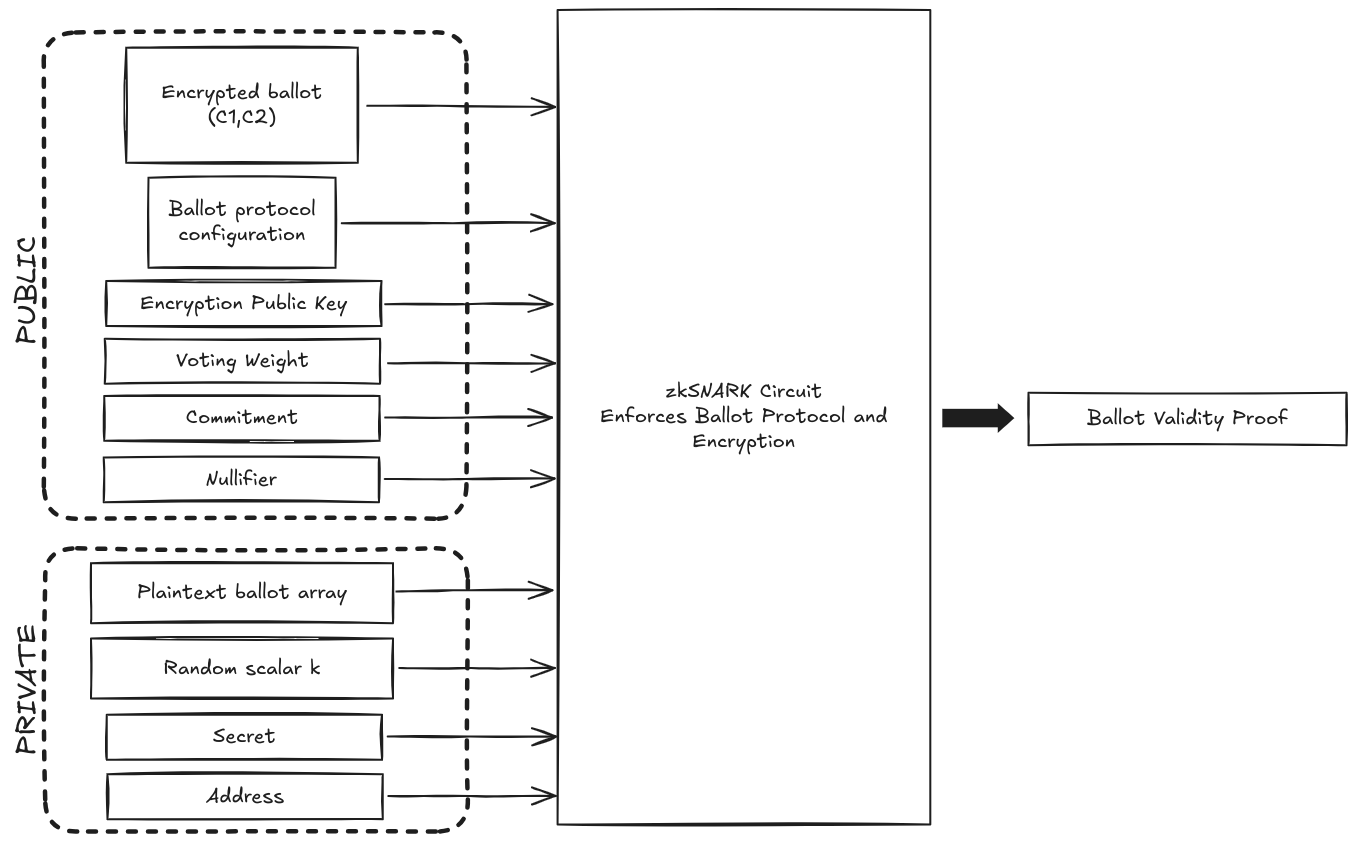
\includegraphics[scale = 0.3, draft = false]{\figs/vote-circuit-inputs.png}}
	\end{figure}
		
	
	\item \textbf{Signature}\\
	
			The \textbf{Signature} authenticates the vote and ensures that it was cast by a legitimate voter. The voter signs necessary components using their private key, depending on the census configuration (e.g., ECDSA, EdDSA, RSA).	
\end{enumerate}
